\documentclass[a4paper,12pt]{article}

\usepackage[slovene]{babel}
\usepackage[utf8]{inputenc}
\usepackage{subfig}
\usepackage{courier}
\usepackage{caption}
\usepackage{graphicx}
\usepackage{amsmath}
\usepackage{tikz}
\usepackage{float}
\graphicspath{{./figures/}}


\title{Poročilo: Community Detection na Microsoft Academics Graphu}
\author{Tim Poštuvan}
\date{\today}

\begin{document}
	\maketitle	
	
	\section{Uvod}
	Naloga raziskovanja je bilo grupiranje institucij iz Microsoft Academics Grapha (MAG) glede na njihovo medsebojno sodelovanje (community detection). 
	
	\section{Potek dela}
	Delo je potekalo v naslednjih korakih:
	\begin{enumerate}
		\item Izdelava grafa
		\item Preizkus različnih metod clusteringa
		\item Analiza dobljenih podatkov
		\item Interpretacija rezultatov
	\end{enumerate}

	\subsection{Izdelava grafa}
	Vozlišča grafa so institucije, povezave pa povezujejo ustanove, ki so sodelovale pri člankih. Utež določene povezave predstavlja število medsebojnih sodelovanj t.j. pri koliko člankih sta ustanovi sodelovali. Članki, pri katerih je sodelovala zgolj ena institucija, se v grafu ne upoštevajo. Tako konstruiran graf je utežen in neusmerjen.
	
	MAG je bil sprva v obliki \textit{(ID članka, leto, IDji institucij)} za vsak članek, kjer \textit{leto} predstavlja leto, v katerem je bil članek napisan, \textit{IDji institucij} pa institucije, ki so pri članku sodelovale. Ta format za obdelavo ni ugoden, zato ga je bilo potrebno pretvoriti v zgoraj opisano obliko (program \texttt{create\textunderscore graph.cpp}). 
	
	\subsection{Preizkus različnih clusteringov}
	Graf sem razdelil na $k$ skupin, za $k = 10$ in $k = 50$. To sem naredil s pomočjo k-spanning tree clusteringa ter spectral clusteringa.
	
	K-spanning tree clustering požrešno izbira največjo povezavo (največja teža) v grafu in clustra, ki sta z njo povezani, poveže skupaj. Če sta vozlišči že v istem clustru, se nič ne zgodi. Opisan postopek ponavlja, dokler je število clustrov večje od želenega. Ker je število povezanih komponent v grafu večje od želenega števila clustrov, bi to pomenilo, da v graf dodamo vse povezave in dobimo clustre, ki so v resnici povezane komponente. Zato sem algoritem modificiral tako, da najprej iz grafa odstrani izolirana vozlišča, naredi k-spanning tree clustering, na koncu pa izolirana vozlišča dodeli enemu izmed že obstoječih clustrov (program \texttt{k\textunderscore spanning\textunderscore tree.cpp}).
	
	Spectral clustering najprej naredi uteženo matriko sosednosti, iz nje pa Laplaceovo matriko. Za to matriko potem izračuna $k$ lastnih vektorjev, ki pripadajo najmanjšim $k$ lastnim vrednostim. Vsako vozlišče nato predstavi s pripadajočo vrstico v Laplaceovi matriki, lastne vektorje pa uporabi kot centre clustrov. Na tako predstavljenem grafu nato naredi clustering s pomočjo k-means clusteringa (program \texttt{spectral\textunderscore clustering.py}).
	
	\subsection{Analiza dobljenih podatkov}
	Na osnovnem grafu sem sprva identificiral najpomembnejše institucije. Mera pomembnosti je utežena stopnjo vozlišča (seštevek uteži povezav, sosednjih temu vozlišču), ki predstavlja določeno institucijo (program \texttt{graph\textunderscore analysis.cpp}).
	
	Ko sem graf razdelil na clustre, sem iz njega izdelal dva nova grafa (program \texttt{create\textunderscore clustered\textunderscore graph.cpp}). Prvi je enak osnovnemu grafu, vendar so iz njega odstranjene vse povezave, ki ne povezujejo dveh vozlišč znotraj clustra. Na tem grafu sem nato za vsak cluster poiskal najpomembnejše institucije (program \texttt{graph\textunderscore analysis.cpp}). S tem sem dobil institucije, ki so najpomembnejša za svoj cluster. Drugi graf pa je ''stisnjen'' osnovni graf. Vse institucije, ki pripadajo istemu clustru, sem združil v eno vozlišče, povezave pa spet predstavljajo medsebojno sodelovanje, vendar tokrat med clustri. Na tem grafu sem pogledal različne statistike:
	\begin{itemize}
		\item število vozlišč
		\item število povezav
		\item povprečna, minimalna in maksimalna utežena stopnja
		\item povprečna, minimalna in maksimalna neutežena stopnja
		\item povprečna, minimalna in maksimalna velikost clustra
	\end{itemize}
	
	Zgoraj napisane statistike z izjemo velikosti clustrov sem naredil tudi na osnovnem grafu. Na njem sem dodatno izrisal še distribucijo uteženih stopenj ter distribucijo uteži povezav v logaritemski skali.
	
	Druge grafe sem tudi vizualiziral s pomočjo NetworkX knjižnice. Uporabil sem krožno predstavitev, saj je edina dala lepo urejeno strukturo grafa. Vozlišča imajo velikost odvisno od števila institucij, ki pripadajo določenemu clustru (velikost je na njih tudi napisana). Povezave imajo debelino odvisno od teže. Oboje zaradi preglednosti ni linearno, vendar logaritmirano. Torej, če je neka povezave $x$-krat debelejša oz. vozlišče $x$-krat večje, to pomeni, da ima na $x$-to potenco večjo težo oz. število institucij glede na drugo vozlišče. Vse povezave imajo debelino v primerjavi z najtežjo povezavo, isto velja tudi za velikosti vozlišč.
	
	\section{Rezultati}
	\subsection{Osnovni graf}
		\begin{figure}[H]
		\centering
		\begin{tabular}{ |c|c| } 
			\hline
			Nodes& 25520 \\
			\hline
			Edges& 4202944 \\
			\hline
			Average weighted degree& 5458.925 \\
			Minimum weighted degree& 0 \\
			Maximum weighted degree& 966443.0 \\
			\hline
			Average degree& 329.3843260188088 \\
			Minimum degree& 0 \\ 
			Maximum degree& 9634 \\
			\hline
		\end{tabular}
		\caption{Statistike grafa}
	\end{figure}

	\begin{figure}[H]
		\centering
		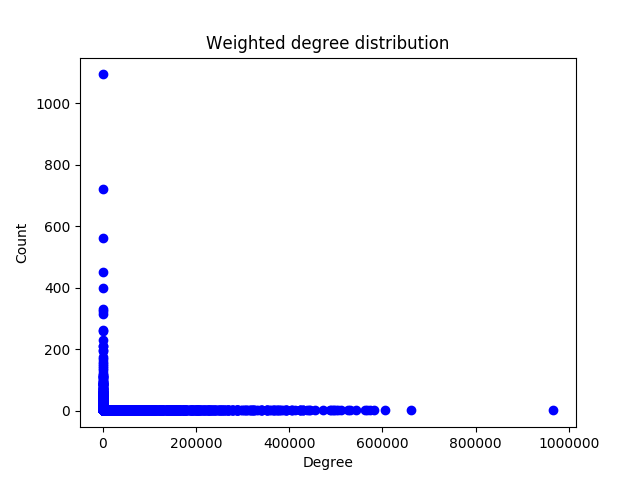
\includegraphics[scale=0.7]{graph_degrees}
		\caption{Distribucija uteženih stopenj}
	\end{figure}

	\begin{figure}[H]
		\centering
		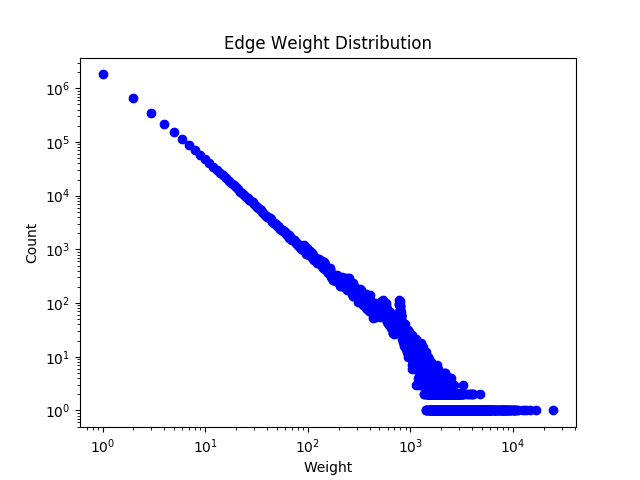
\includegraphics[scale=0.7]{graph_edge_weights}
		\caption{Distribucija uteži povezav}
	\end{figure}

	\subsection{K-spanning tree clustering ($k = 10$)}
	\begin{figure}[H]
		\centering
		\begin{tabular}{ |c|c| } 
			\hline
			Nodes& 10 \\
			\hline
			Edges& 8 \\
			\hline
			Average weighted degree& 2.0 \\
			Minimum weighted degree& 0  \\
			Maximum weighted degree& 10.0 \\
			\hline
			Average degree& 1.6 \\
			Minimum degree& 0 \\ 
			Maximum degree& 8 \\
			\hline
			Average cluster size& 2552.0 \\
			Minimum cluster size& 1 \\
			Maximum cluster size& 25509 \\
			\hline
			
		\end{tabular}
		\caption{Statistike grafa}
	\end{figure}
	
	\begin{figure}[H]
		\centering
		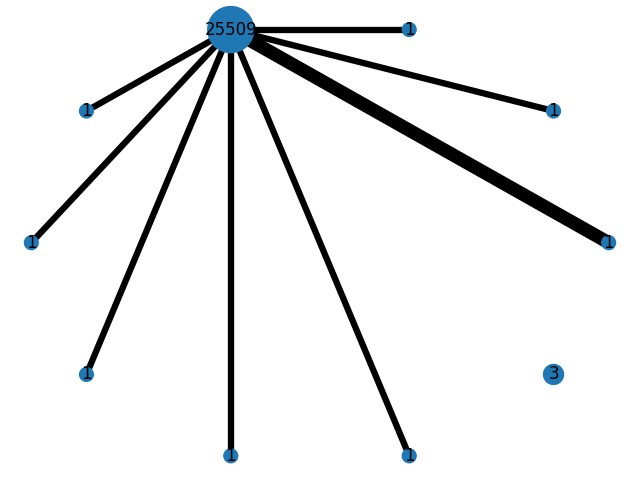
\includegraphics[scale=0.7]{spanning_merged_graph_10_visualization}
		\caption{Vizualizacija grafa}
	\end{figure}


	\subsection{K-spanning tree clustering ($k = 50$)}
	\begin{figure}[H]
		\centering
		\begin{tabular}{ |c|c| } 
			\hline
			Nodes& 50 \\
			\hline
			Edges& 48 \\
			\hline
			Average weighted degree& 4.48 \\
			Minimum weighted degree& 0  \\
			Maximum weighted degree& 112.0 \\
			\hline
			Average degree& 1.92 \\
			Minimum degree& 0 \\ 
			Maximum degree& 48 \\
			\hline
			Average cluster size& 510.4 \\
			Minimum cluster size& 1 \\
			Maximum cluster size& 25467 \\
			\hline
			
		\end{tabular}
		\caption{Statistike grafa}
	\end{figure}	
	
	\begin{figure}[H]
		\centering
		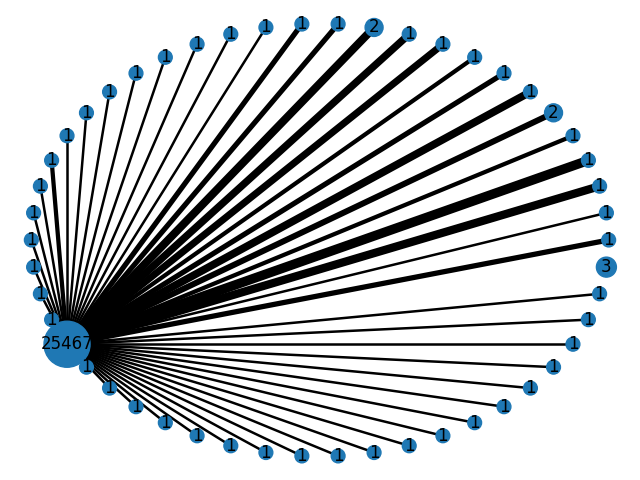
\includegraphics[scale=0.7]{spanning_merged_graph_50_visualization}
		\caption{Vizualizacija grafa}
	\end{figure}


	\subsection{Spectral clustering ($k = 10$)}
	\begin{figure}[H]
		\centering
		\begin{tabular}{ |c|c| } 
			\hline
			Nodes& 10 \\
			\hline
			Edges& 18 \\
			\hline
			Average weighted degree& 2989866.8 \\
			Minimum weighted degree& 0  \\
			Maximum weighted degree& 13647669.0 \\
			\hline
			Average degree& 3.6 \\
			Minimum degree& 0 \\ 
			Maximum degree& 8 \\
			\hline
			Average cluster size& 2552.0 \\
			Minimum cluster size& 2 \\
			Maximum cluster size& 14315 \\
			\hline
			
		\end{tabular}
		\caption{Statistike grafa}
	\end{figure}
	
	\begin{figure}[H]
		\centering
		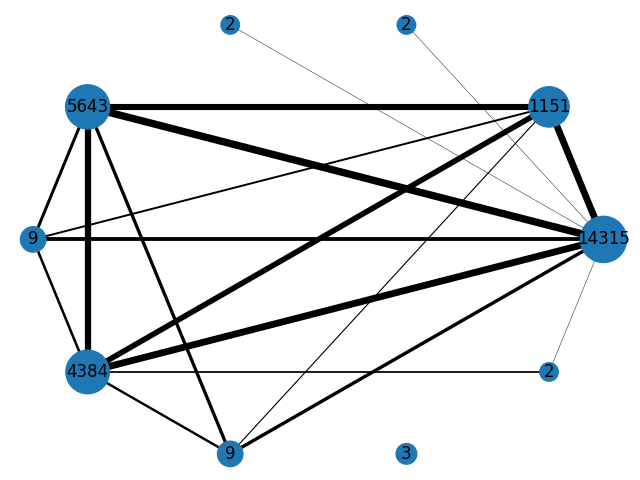
\includegraphics[scale=0.7]{spectral_merged_graph_10_visualization}
		\caption{Vizualizacija grafa}
	\end{figure}


	\subsection{Spectral clustering ($k = 50$)}
	\begin{figure}[H]
		\centering
		\begin{tabular}{ |c|c| } 
			\hline
			Nodes& 49 \\
			\hline
			Edges& 481 \\
			\hline
			Average weighted degree& 1549392.0 \\
			Minimum weighted degree& 0  \\
			Maximum weighted degree& 18101874.0 \\
			\hline
			Average degree& 19.632653061224488 \\
			Minimum degree& 0 \\ 
			Maximum degree& 42 \\
			\hline
			Average cluster size& 520.8163265306123 \\
			Minimum cluster size& 2 \\
			Maximum cluster size& 7673 \\
			\hline
			
		\end{tabular}
		\caption{Statistike grafa}
	\end{figure}
	
	\begin{figure}[H]
		\centering
		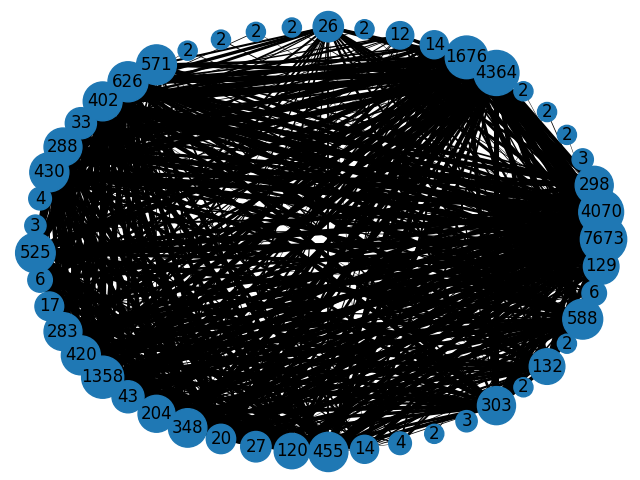
\includegraphics[scale=0.7]{spectral_merged_graph_50_visualization}
		\caption{Vizualizacija grafa}
	\end{figure}
	
	\section{Interpretacija rezultatov}	
	\subsection{Osnovni graf}
	
	Osnovni graf je precej velik, saj ima več kot $25\; 000$ vozlišč in $420\; 000$ povezav. Povprečna neutežena stopnja vozlišč je $329.38$, kar je ogromno. Tak graf je zelo tesno povezan in sodi med tako imenovane \textit{small-world networke} (povprečna neutežena razdalja med vozlišči je precej majhna). Uteži povezav so po večini bolj majhne -- število sodelovanj med istim parom institucij ni tako veliko, kar tudi ni nič nepričakovanega. Graf ima zelo velik razpon uteženih stopenj vozlišč s povprečjem $5458.93$. Večina stopenj je relativno majhnih, vendar obstajajo tudi vozlišča z zelo veliko uteženo stopnjo. Tem vozliščem se reče \textit{hubi} in so v našem primeru najpomembnejši, saj predstavljajo jedra communityjev. Glede na zgoraj omenjeno mero so najpomembnejša vozlišča osnovnega grafa (datoteka \texttt{most\textunderscore important\textunderscore institutions.txt}):
	\begin{itemize}
		\item Harvard University
		\item Centre national de la recherche scientifique
		\item Max Planck Society
		\item Johns Hopkins University
		\item University of Washington		
	\end{itemize}
	
	\subsection{K-spanning tree clustering}
	K-spanning tree clustering je za oba $k$ zgradil zvezdi podoben graf. Clustering na prvi pogled izgleda zelo uspešen, saj je v grafu malo povezav, te pa imajo celo zelo majhno težo. Povprečna teža povezave (pri $k = 10$) je zgolj $2.0$, maksimalna pa samo $10.0$. To je po kriteriju, da imajo povezave znotraj clustra čim večjo težo, med clustri pa čim manjšo, skoraj idealno.
	Težavo opazimo, če pogledamo velikosti clustrov. Vidimo, da ima največji cluster (pri $k = 10$) $25509$ vozlišč od skupno $25520$, kar je $0.9996\%$ vseh vozlišč. Tudi za druge $k$ je situacija podobna, kar pomeni, da ima graf zelo tesno povezano jedro, ostale institucije pa so zgolj povezne nanj. Na takih grafih k-spanning tree clustering ne deluje dobro, saj bomo vedno dobili eno veliko jedro, ostalo pa bodo zelo majhni clustri, povezani na to jedro. V sekciji Nadaljnje raziskovanje bom tudi opisal modifikacijo algoritma, s katero bi se rezultat verjetno dalo izboljšati.
	
	\subsection{Spectral clustering}
	Spectral clustering je dal veliko boljši rezultat od k-spanning tree clusteringa. Algoritem je veliko bolj smiselno naredil communityje, čeprav se potem tu pojavi vprašanje, če jih je res smiselno razcepiti. Maksimalna utežena stopnja vozlišča (pri $k=10$) je več kot $10^7$, kar je glede na distribucijo uteži povezav ogromno -- maksimalna teža povezave je zgolj malo manj kot $25\;000$. Tudi iz vizualizacije hitro vidimo, da so največja $4$ vozlišča med seboj testno povezana in bi se jih dalo združiti skupaj. Algoritem je naredil več clustrov večjih velikosti ($4$ imajo več kot $1\;000$ institucij), saj teži k bolj uravnoteženim velikostim. Premajhni in preveliki clustri so tu kaznovani, pri k-spanning tree clusteringu pa ne, zato je pri slednjem velika neuravnovešenost. Kljub vsemu je po podrobnejši analizi najpomembnejših institucij clustrov viden vzorec. Izsek najpomembnejših institucij v clustrih za $k=10$ (datoteka \texttt{most\textunderscore important\textunderscore institutions\textunderscore in\textunderscore clusters\textunderscore 10.txt}).
	
	\hspace{1cm}
	
	Cluster 0 (size 14315):
	\begin{itemize}
		\item Harvard University 866588
		\item Centre national de la recherche scientifique 586051
		\item Max Planck Society 536439
		\item Johns Hopkins University 517678
		\item Ohio State University 508367
	\end{itemize}

	\hspace{1cm}	
	
	Cluster 1 (size 1151):
	\begin{itemize}
		\item University of Tokyo 176845
		\item Kyoto University 117612
		\item Osaka University 102749
		\item Tohoku University 93317
		\item Nagoya University 86013
	\end{itemize} 
	
	\hspace{1cm}
	
	Cluster 4 (size 5643):
	\begin{itemize}
		\item Chinese Academy of Sciences 274349
		\item University of Sydney 111107
		\item National Taiwan University 88964
		\item Peking University 87924
		\item University of Queensland 82510
	\end{itemize}

	\hspace{1cm}
	
	Cluster 6 (size 4384):
	\begin{itemize}
		\item Seoul National University 80789
		\item Yonsei University 54386
		\item Hanyang University 31957
		\item Pusan National University 27119
		\item University of Ulsan 24076
	\end{itemize}

	
	Iz izseka je jasno razvidno, kako so glavne institucije povezane. Glavne institucije Clustra 1 so vse na Japonskem, pri Cluster 6 pa iz Južne Koreje. V Clustru 4 gre za kitajske in avstralske ustanove, torej je smiselno sklepati, da so tudi ostale institucije iz jugovzhodne Azije in Avstralije. Še vedno nejasno razdeljen community je Cluster 0, saj ni vidno, zakaj se je algoritem odločil ravno za tako delitev.
	
	Da bi Cluster 0 še bolj razdelil, sem naredil spectral clustering za $k = 50$. Izgled grafa tukaj sploh ni obetaven, saj se vse zdi povezano med seboj. Vendar se pri analizi clustrov izkaže, da je nastalo več smiselnih clustrov. Izsek najpomembnejših institucij v clustrih za $k=50$, ki se niso bile razvidne pri $k=10$ (datoteka \texttt{most\textunderscore important\textunderscore institutions\textunderscore in\textunderscore clusters\textunderscore 50.txt}).
	
	\hspace{1cm}
	
	Cluster 0 (size 7673):
	\begin{itemize}
		\item Harvard University 441519
		\item University of Washington 259538
		\item Johns Hopkins University 250583
		\item University of Michigan 233097
		\item University of Pennsylvania 222116
	\end{itemize}
	
	\pagebreak
	
	Cluster 1 (size 4070):
	\begin{itemize}
		\item University of Melbourne 135593
		\item University of Oxford 133319
		\item University College London 131208
		\item University of Cambridge 130062
		\item University of Sydney 125614
	\end{itemize}
	
	\hspace{1cm}
	
	Cluster 7 (size 4364):
	\begin{itemize}
		\item Centre national de la recherche scientifique 291045
		\item Max Planck Society 263034
		\item Spanish National Research Council 171873
		\item Heidelberg University 156829
		\item University of Manchester 149225
	\end{itemize}

	Cluster 20 (size 33):
	\begin{itemize}
		\item Lutheran School of Theology at Chicago 16
		\item Wartburg Theological Seminary 13
		\item George Fox Evangelical Seminary 12
		\item Luther Seminary 12
		\item Columbia Theological Seminary 11
	\end{itemize}


	Vidimo, da je graf bolje razdeljen. Sedaj so v Clustru 0 ameriške univerze in evropske v Clustru 7 (pri $k=10$ je bilo vse skupaj v Clustru 0). Od Evrope so nekoliko ločene angleške institucije, ki sodelujejo z avstralskimi (Cluster 1). V celotni datoteki je še nekaj primerov clustrov, ki so lepo geografsko povezani. V Clustrih 43 in 49 je vidno sodelovanje znotraj Indije ter v Clustru 47 znotraj Brazilije. Cluster 20 je zanimiv, ker edini ni povezan zaradi geografskih značilnosti. Vse glavne institucije clustra se ukvarjajo s teologijo, kar pomeni, da jih združuje raziskovalno področje. 
	
	\section{Nadaljnje raziskovanje}
	
	Problem community detectiona je zelo obširen, zato obstaja še mnogo stvari, katere bi se dalo narediti. Tukaj bom na kratko opisal zgolj nekaj idej.
	
	Najprej nadgradnja trenutnih algoritmov. Dobro bi bilo poskusiti še druge vrednosti $k$. Morda stvar razpade na bolj smiselno clustre, če naredimo več ali manj clustrov.
	
	Naslednja izboljšava, ki se nanaša predvsem na pomanjkljivost k-spanning tree clusteringa, je redčenje grafa. Glavni problem za neuspešnost algoritma je, da imamo zelo tesno povezano jedro, ostala vozlišča pa so povezana nanj. Zato algoritem pusti jedro pri miru, osami pa ostala vozlišča. To je ravno v nasprotju z našim namenom, saj želimo razdeliti jedro. Predlagam, da bi iz grafa na začetku odstranili vsa vozlišča, ki niso v jedru. Nato bi jedro razdelili na $k$ clustrov in na koncu odstranjena vozlišča dodali najprimernejšemu že obstoječemu clustru. 
	
	Vsekakor bi na danem grafu lahko poskusili še druge algoritme in embeddinge grafov. Gotovo bi bilo dobro preizkusiti node2vec v kombinaciji s k-means clusteringom. Vredno bi bilo poskusiti tudi drug princip clusteringa. Pri mojem raziskovanju sem uporabljal zgolj hard clustering (vsako vozlišče je element zgolj enega clustra), lahko pa bi poskusili še soft clustering (vozlišče je lahko element večih clustrov).
	
	Zanimivo bi bilo pogledati problem še iz malenkost drugačnega zornega kota. Lahko bi gledali spreminjanje communityjev skozi čas. Prav tako bi lahko analizirali samo communityje na posameznem področju, saj se sodelovanja institucij na različnih področjih lahko zelo razlikujejo. 
		
	Zadnji predlog se nanaša na vrednotenje uspešnosti clustrov. Pri mojem raziskovanju sem uspešnost clusteringa ovrednotil predvsem glede na geografsko povezanost. Zelo verjetno to ni edini smiseln kriterij, tako da bi se lahko spomnili še drugih načinov. Primer je sodelovanje institucij, ki se ukvarjajo predvsem z neko panogo (npr. če so v clustru samo institucije, katerih glaven fokus je matematika, bi bila to dobra delitev).
		
\end{document}
